\chapter{Speicher}





\section{Realisierung Heuristik Agent}
%Realisierung nicht lernender Agent / feste Strategie
Der vorausschauende Heuristik Agent ist ein nicht lernender Agent der eine von uns festgelegte Strategie erhält. Die Strategie besteht aus einer Stellungsbewertung (Heuristik) und einer 2 Spielzüge vorausschauenden Spielbaumsuche. Wir werden in Abschnitt \ref{Spieltheorie} Spieltheorie die Theoretischen Grundlagen erklären, die wir für die Implementierung des vorausschauenden Heuristik Agenten benötigen.  


In der Implementierung des vorausschauenden Heuristik Agenten ist, neben der Bewertungsfunktion, noch ein anderes Verfahren enthalten. Das Suchbaumverfahren für 2-Personenspiele. Dieses Verfahren durchsucht einen Spielbaum nach der bestmöglichen Aktion (einem Spielzug) in einem gegebenen Zustand. Ein Zustand oder Spielzustand ist eine Spielsituation bzw. eine Stellung der Spielfiguren auf dem Spielfeld. \\

Das Problem der Suchverfahren ist die Dimensionalität bzw. Komplexität des Ausgangsproblems. Suchbaumverfahren können für sehr einfache Probleme relativ schnell eine optimale Aktion finden. Die Größe des Suchbaums wächst exponentiell mit der Komplexität des Problems, d.h. die Laufzeit des Suchbaumverfahrens ohne Erweiterungen könnte für das Strategiespiele Tic Tac Toe nicht handhabbar sein und ist für das Strategiespiel Reversi nicht handhabbar. Wir schreiben ''könnte'' bei Tic Tac Toe, weil dieses noch ein recht einfacher Vertreter der Strategiespiele ist, dahingegen ist Reversi ein komplexeres Strategiespiel. \\

Um die Diemensionalitätsproblematik zu lösen, kombinieren wir Suchbaumverfahren mit Heuristiken, wir bezeichnen diese Kombination als heuristische Suche. Eine Heuristik berechnet eine Gewinnwahrscheinlichkeit, ausgehend von einem Spielzustand. Ein Spielzustand mit einer hohen heuristischen Bewertung ist, gegenüber einem Spielzustand mit niedriger heuristischer Bewertung, zu bevorzugen. \\

Das Suchbaumverfahren muss den Suchbaum, unter Verwendung einer Heuristik, nicht mehr komplett durchsuchen. Die Suche kann in einer bestimmten Suchbaumtiefe abgebrochen werden. Das Suchbaumverfahren liefert die erste Aktion einer Aktionssequenz. Eine Aktionssequenz ist eine Folge von Aktionen und beschreibt einen Pfad im Suchbaum. Die Aktionssequenz, welche von der heuristischen Suche ausgewählt wurde, repräsentiert den Spielzustand mit der maximalen Gewinnwahrscheinlichkeit. \\

Die Qualität dieser Gewinnschätzung ist wiederum von der maximalen Suchtiefe und der Bewertungsfunktion abhängig. Eine größere Suchtiefe resultiert in einer besseren Schätzung, weil unter Umständen mehr Spielzustände berücksichtigt werden können. Die Verwendung einer Bewertungsfunktion ist keine Garantie für eine optimale Strategie. Verschiedene Bewertungsfunktionen können stark voneinander abweichende Gewinnschätzungen für Spielzustände berechnen. \\

\section{Realisierung des TD-Q lernenden Agent}


Wie realisiert das TD-Q-Lernen diesen verstärkenden Lernansatz? Das TD-Q-Lernen lernt Q-Werte für Zustand/Aktionspaare, diese Q-Werte werden bei jedem erneuten Auftreten des Zustand/Aktionspaares aktualisiert. Eine Q-Funktion ist eine Abbildung von allen möglichen Zustand/Aktionspaaren auf Q-Werte und eine Q-Funktion ist eine Möglichkeit Nutzeninformationen zu speichern \cite[974]{Russell}. Nachdem der Agent eine Q-Funktion gelernt hat, kann er mittels dieser, vermeintlich optimale Aktionen auswählen. Wir schreiben ''Vermeintlich'', weil eine gelernte Q-Funktion nicht immer zu einer optimalen Strategie konvergiert.

Wir zeige in dieser Arbeit praktisch, dass das TD-Q-Lernen ohne Erweiterungen, nur auf Probleme mit geringer Komplexität angewendet werden kann. Die Komplexität bzw. Dimensionalität des Ausgangsproblems ist ein Grund dafür, dass die gelernte Q-Funktion nicht immer zu einer optimalen Strategie konvergiert, ein anderer Grund ist die zeitliche Beschränkung durch die Realität, d.h. in der Realität können nicht unendlich viele Testspiele durchgeführt werden. Es wurde bereits empirisch belegt, dass das Q-Lernen, sollte jedes Zustand/Aktionspaar nahezu unendlich oft besucht und aktualisiert werden, immer zu einer optimalen Strategie konvergiert. Das Problem dabei ist, dass die Komplexität bzw. die Dimensionalität des Ausgangsproblems, ein exponentiellen Verhältnis zur Zustands- und Aktionsmenge hat. \\

Lernt der TD-Q Agent, z.B. innerhalb von 10.000 Testspielen eine nahezu optimale Strategie für ein Tic Tac Toe Spiel mit 3 mal 3 Dimensionen (9 Spielfelder), dann ist das TD-Q-Lernen praktisch für ein Strategiespiel bis zu dieser Dimensionalität anwendbar. Erhöhen wir die Zustands- und Aktionsdimension, z.B. bei einem 16 Spielfelder Tic Tac Toe Spiel, dann reichen selbst 1.000.000 Testspiele unter Umständen nicht mehr aus, um eine annähernd optimale Strategie zu lernen. Jede weitere Dimension erhöht außerdem die Dauer eines Trainingsspiels, d.h. für jede weitere Dimension benötigt das TD-Q-Lernverfahren erheblich mehr Testspiele, um zu einer annähernd optimalen Strategie zu konvergieren und gleichzeitig erhöht sich die Dauert jedes Testspiels für jede zusätzliche Dimension des Ausgangsproblems.

\section{Spieltheorie}


Im Unterkapital Spieltheorie (Abschnitt \ref{sec:Spieltheorie}) werden uninformierte Suchbaumverfahren, deren Optimierungsmöglichkeiten, Übergangstabellen und Heuristiken erklärt.\\

Die Minimax-Suche (Abschnitt \ref{subsec:Minimax}) ist ein uninformiertes Suchbaumverfahren. Die Minimax-Suche kann in Zweipersonenstrategiespielen eingesetzt werden, um eine optimale Strategie zu finden. In der Praxis ist das Verfahren jedoch nicht anwendbar. Die Suchbäume realistischer Probleme sind meist entartet bzw. zu groß für eine klassische Minimax-Suche. Die Alpha-Beta-Kürzung (Abschnitt \ref{subsec:Alpha-Beta-Kürzung}) ist eine Verbesserung der Minimax-Suche, dieses Optimierungsverfahren Versucht, den meist viel zu großen Suchbaum zu kürzen, ohne das Endergebnis der Minimax-Suche zu beeinflussen. Wir werden die Minimax-Suche bzw. Alpha-Beta-Suche für die Implementierung des Heuristik Agenten verwenden. Die iterativ vertiefende Tiefensuche (Abschnitt \ref{subsec:Iterativ vertiefende Tiefensuche}) ist ein uninformiertes Suchverfahren, welches Breitensuche und Tiefensuche kombiniert und bis zu einer bestimmten Suchtiefe ein bestmögliches Ergebnis sucht. Wir verwenden die iterativ vertiefende Tiefensuche, für die Verbesserung der vorausschauenden Suche des Heuristik Agenten. \\

Die Übergangstabellen (Abschnitt \ref{subsec:Übergangstabellen}) beschreiben eine Möglichkeit Übergänge zu vermeiden. Übergänge sind identische Spielsituationen, die durch unterschiedliche Aktionssequenzen (eine Folge von Spielzügen) dargestellt werden können, daher scheinen die Spielsituationen unterschiedlich zu sein. Das Zobrist-Hash Verfahren beschreibt eine Möglichkeit die Spielsituationen eindeutig als Zahlwerte darstellen zu können. Wir verwenden dieses Hashverfahren bzw. auch eine Art der Übergangstabellen für das TD-Q lernen. \\

Heuristiken bilden die stärkste Leistungsverbesserung, bezüglich der Rechenzeit, für Suchbaumverfahren. Eine Heuristik (Abschnitt \ref{subsec:Heuristik}) ist eine Bewertungsfunktion B(s), welche für jeden Spielzustand (Stellung der Spielfiguren) s eine Schätzung bereitstellt. Die Schätzung gibt an, wie hoch die Gewinnchance, in einem bestimmten Spielzustand, für den Spielzug ausführenden Spieler, ist. Heuristiken ermöglichen das abbrechen der Suche innerhalb eines Suchbaumes, d.h. auch die nicht Blattkonten des Baumes können Spielergebnisse bereitstellen. Die Kombination von uninformierter Suche und Heuristiken ist nicht mehr uninformiert. Heuristiken stellen zusätzliche Spielinformationen bereit. Die Literatur bezeichnet dies daher als heuristische (informierte) Suche \cite[105]{Ertel}. \\

Wir fassen zusammen: Die Implementierung des Heuristik Agenten erhält eine iterativ vertiefende Alpha-Beta Suche, diese kann auch nicht Blattknoten des Suchbaums, mittels einer Heuristik, bewerten. Wir können also die Rechenzeit des Heuristik Agenten begrenzen, indem wir die maximale Suchtiefe auf 2 Halbzüge begrenzen. Der Heuristik Agent expandiert, wie die iterativ vertiefende Tiefensuche, zu erst alle Knoten in einer Tiefe und erhöht danach schritt für schritt (iterativ) die aktuelle Tiefenschranke, bis zu der maximal möglichen Tiefe. 

\section{Spieltheorie}
\label{sec:Spieltheorie}
In diesem Abschnitt werden wir erklären was uninformierte Suchbaumverfahren, Übergangstabellen und Heuristiken sind. Wir verwenden diese Methoden, aus der Spieltheorie, für die Implementierung unserer Agentenmodelle. Wolfgang Ertel beschreibt Spiele mit Gegenspieler wie folgt \cite[114]{Ertel}: \\ 

Schach, Vier gewinnt, Dame, Tic Tac Toe und Reversi sind strategische Spiele für zwei Personen, die gegeneinander antreten, um nach den Regeln des Spiels, den Gegenspieler zu besiegen. Diese Spiele sind deterministisch, weil das Spiel nicht vom Zufall abhängt und der gleiche Spielzug führt, bei gleichem Ausgangszustand, immer zum selben Spielergebnis. Ein nichtdeterministisches Spiel mit Gegenspieler ist z.B. Backgammon, denn Würfelergebnisse und somit der Zufall sind Bestandteil des Spiels. Die eben genannten Strategiespiele sind alle vollständig beobachtbar (wir verfügen über vollständige Information). Sie sind vollständig überschaubar, weil zu jedem Zeitpunkt des Spiels, das Spielfeld und alle Spielzüge einsehbar sind. Ein nicht vollständig beobachtbares Spiel ist, z.B. Poker oder andere Kartenspiele. Bei einem Poker Spiel sind die gegnerischen Karten und die Karten im Spieldeck unbekannt.\\

''In der künstlichen Intelligenz haben die gebräuchlichsten Spiele in der Regel eine spezielle Natur - die Spieltheoretiker sprechen von deterministischen Zwei-Personen-Nullsummenspielen mit vollständiger Informaiton, bei denen zwei Spieler abwechselt agieren (wie zum Beispiel Schach) \cite[206]{Russell}.'' Die von Russell und Norvig erwähnten Eigenschaften treffen auch auf unsere Strategiespiele zu. Reversi und Tic Tac Toe sind deterministische und vollständig überschaubare Nullsummenspiele, d.h. wir müssen zufällig auftretende Zustandsübergänge und unbekannte Informationen, in unseren Heuristiken und Lernverfahren, nicht berücksichtigen. Nullsummenspiel bedeutet: gewinnt ein Spieler eine Partie, dann verliert der Gegenspieler automatisch in gleicher Höhe.












Bezüglich der extrem hohen Rechenzeit , müssen wir eine weitere Komponente dazunehmen, das uninformierte Suchverfahren der iterativ vertiefenden Tiefensuche.

Eine Heuristik ist eine Bewertungsfunktion für Spielzustände. Die Bewertungsfunktion gibt an, wie gut oder schlecht eine bestimmte Spielsituation ist. \\

''Heuristiken sind Problemlösungsstrategien, din in vielen Fällen zu einer schnelleren Lösung führen als die uninformierte Suche. Es gibt jedoch keine Garantie hierfür. Die heuristische Suche kann auch viel mehr Rechenzeit beanspruchen und letztlich dazu führen, dass die Lösung nicht gefunden wird.  \cite[105]{Ertel}''\\






















\subsection{Übergangstabellen}
\label{subsec:Übergangstabellen}
Eine Übergangstabelle (eng. transition table) ist eine Tabelle in der Spielsituationen mit verschiedenen Attributen gespeichert werden (vgl. \cite[215\psq]{Russell}). Übergänge sind der Grund dafür, dass der gleiche Spielzustand durch unterschiedliche Spielzugsequenzen auftritt (siehe Abbildung \ref{fig:transitionen_tictactoe}). \\

\begin{figure}[!htbp]
  \centering
  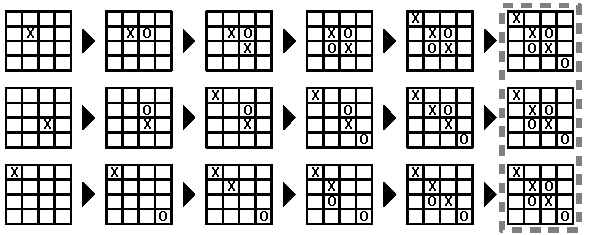
\includegraphics{inhalt/abbildungen/transitionen_tictactoe.pdf}
  \caption{Verschiedene Spielzugsequenzen enden im selben Spielzustand.}
  \label{fig:transitionen_tictactoe}
\end{figure} 

Übergänge innerhalb des Suchbaums verursachen Redundanzen. Für jede dieser Redundanzen wird eine erneute Suche durchgeführt, falls diese nicht durch Alpha-Beta-Kürzung abgeschnitten werden. Sollten diese Übergänge vermieden werden können, dann würde sich die Rechenzeit der Suchverfahren weiter verringern, weil weniger Spielzustände durchsucht bzw. expandiert werden müssen. \\

Wir können uns das TD-Q-Lernen, als eine Art Übergangstabelle vorstellen. Die Tabelle würde 3 Spalten haben. Die erste Spalte beinhaltet den Spielzustand, die zweite Spalte die dazugehörige Aktion und die dritte Spalte enthält den Q-Wert (Nutzwert), d.h. Zustand/Aktionspaare werden auf Q-Werte abgebildet. Diese Tabelle wird nicht unbedingt geführt um Redundanzen zu vermeiden, sondern eher um Nutzeninformationen zu speichern.

















Bei diesen Problemen ist dem Agenten der direkte Nutzen des Aktionsergebnisses nicht bekannt, erst nach einer Folge von Aktionen (am ende des Spiels) wird dem Agenten eine Belohnung zugeteilt (vgl. \cite[397]{Alpaydin}). \\

Dies trifft auch auf die Strategiespiele Tic Tac Toe und Reversi zu, denn bei diesen Spielen erhält der Agent keine direkte Belohnung nach den einzelnen Spielzügen. Erst am Ende eines Spiels entsteht ein Sieg, eine Niederlage oder ein Unentschieden und der Agent erhält dem entsprechen eine verspätete Belohnung. \\ 






















Die Testergebnisse des vorausschauenden Heuristik Agenten gegen den Zufallsagenten sind eindeutig. Der kleinste Erfolg des Heuristik Agenten, mit 64\% Gewinnquote bestätigt bereits die Hypothese aus Abschnitt \ref{sec:Ergebnisse}. Die größte Gewinnquote des von uns implementierten Tic Tac Toe vorausschauenden Heuristik Agenten ist 100\%, d.h. von 100 Testspielen in einem 16 Spielfelder Tic Tac Toe, wenn der Heuristik Agent das Spiel beginnt, gewinnt der Heuristik Agent alle 100 Testspiele. \\

Die Testspiele der gelernten TD-Q-Strategien gegen den vorausschauenden Heuristik Agent sind sehr eindeutig ausgefallen. Jede gelernte Strategie, egal ob für das 9 oder 16 Spielfelder Tic Tac Toe, spielt gegen die nicht gelernte Strategie des vorausschauenden Heuristik Agenten immer das selbe Spiel. Der vorausschauende Heuristik Agent führt ebenfalls immer die selben Spielzüge aus. Die folge daraus ist, beide Agenten spielen in 100 Testspielen immer die exakt gleiche Partie mit dem selben Spielergebnis. Die gelernten Strategien haben es zudem nicht geschafft, innerhalb von maximale 10.000 Trainingsspielen, eine Strategie zu lernen, die den vorausschauenden Heuristik Agenten besiegt. \\

Die einzige Ausnahme war die in 1.000 Testspielen gelernte Strategie, diese erreichte 100 unentschieden gegen den nachziehenden Heuristik Agent (jeweils im 9 und 16 Spielfelder Tic Tac Toe). Alle 100 Testspiele wurden von beiden Agenten exakt gleich gespielt. Für die Tests wäre es vermutlich interessanter einen weiteren Trainingsmodus für den TD-Q-Agenten zu implementieren. Ein Trainingsmodus der nicht gegen sich selbst spielt, sondern gegen Andere Agenten. Die Testergebnisse gegen den Heuristik Agenten würden dann wahrscheinlich auch variieren, dies ist jedoch kein Ziel dieser Arbeit. \\

Die Testergebnisse in Spielen gegen den Zufallsagenten sind ebenfalls kritisch zu betrachten, denn sie hängen offensichtlich vom Zufall ab. Wir können die Testergebnisse demnach nur berücksichtigen, wenn diese eindeutig sind, d.h. die gelernten Strategien müssten hohe Gewinnquoten und niedrige Verlustquoten erreichen. Wir versuchen trotzdem die Leistungsfähigkeit des TD-Q-Lernens, über die Testergebnisse, gegen den Zufallsagenten, herzuleiten. \\ 